
\subsection{\label{sec:Runtime}Runtime System}

The runtime system is the module that is responsible for managing
all the data in a data model instance at runtime. This includes the
following tasks:
\begin{itemize}
\item \textbf{Data Containment: }Holding data that make up the current state
of a running data model instance, which includes all entities and
connections between entities.
\item \textbf{Index Containment:} Keeping and updating all indexes on the
data model instance.
\item \textbf{Transaction Execution:} Making sure that all transactions
are executed correctly.
\item \textbf{Data Persistence:} Taking care of the persistence of the data
model instance. 
\end{itemize}
The runtime implements a series of runtime interfaces, used by the
generated code. There could be many different implementations of the
runtime interface, each with different strategies and solutions on
how to solve these tasks. This way it is easy to switch between different
runtime implementations without any changes to the generated code,
or to the code written by the users.


\subsubsection{Runtime Interface}

In the creation of the runtime interface we have tried to make it
independent of how it would be implemented.

Since the runtime interface is non-generated code, it has no knowledge
of specific data models at compile time. It gets the information about
the specific data model that it should manage from the meta model
instance at runtime. Thus, in the runtime interface specific kinds,
relations and indexes are referred to by their index in the meta model
instance.

The runtime interface consists of a number of Java interfaces that
a runtime implementation must implement. These interfaces are:
\begin{itemize}
\item \texttt{IRuntimeFactory} - Given the meta model instance for a specific
data model it returns an \texttt{IDataModelInstanceFactory}
\item \texttt{IDataModelInstanceFactory} - Can load, create and delete individual
instances of a data model.
\item \texttt{IDataModelInstance} - Represents an instance of a data model.
Has methods to start and stop the instance and execute views and actions.
\item \texttt{IView} - Represents a view on the data model implemented by
the user.
\item \texttt{IAction} - Represents an action on the data model implemented
by the user.
\item \texttt{IResult} - Represents the result of executing a view or an
action on the data model instance.
\item \texttt{IDataModelView} - This is the interface that the user implementations
of actions are bound to through the auto-generated internal API interfaces
and classes.
\item \texttt{IDataModelUpdate} - This is the interface that the user implementations
of views are bound to through the auto-generated internal API interfaces
and classes.
\item \texttt{IIndex} - Represents an index on the data model.
\item \texttt{IEntity} - Represents an entity in the data model.
\end{itemize}
Any implementation of an EDMA runtime system must provide these interfaces
for the generated code to bind up against.


\subparagraph{Procedural vs Declarative Query Languages}

In EDMA queries to the data models are written in a procedural manner,
where the user describes an algorithm for how to construct the result,
using the structure of the data model to navigate and using set operations
to narrow or widen the result.

In SQL, queries are written in a declarative way, where the user describes
what the result should be, but not how to obtain it.

It is a subjective matter which of these approaches that feel most
natural, but if a user has an object oriented background, he is used
to get things done in a procedural manner.

One advantage of the declarative approach is that the underlying system
has freedom to analyze the query and try to find the most optimal
algorithm for creating the result.

But even though EDMA takes a procedural approach to obtain the result,
we can use abstraction to let the runtime system delay decisions and
do some amount of optimization on its own. One example of this is
the way sets and set operations are handled in the runtime system.


\subparagraph{Sets and set operations}

One of the important features the runtime system most provide is set
operations such as union, intersection and subtraction. But instead
of representing a set by a java class, we simply use an index that
the runtime system controls. In this way when the user asks the runtime
system to perform an intersection of two sets, all the runtime system
actually gets are the indexes of the sets to intersect and it returns
a new index that represents the intersection of the sets. But the
runtime does not actually have to perform the intersection at this
time. Only when the user actually wants to access or count the elements
in the set, the runtime must perform the intersection. In the case
of complicated queries that involves many set operations before the
final result is produced, the runtime system can analyze and optimize
how to perform these set operations. This method of postponing evaluation
until the result is actually used is known as lazy evaluation.

Especially in a runtime implementation that is backed by an SQL database,
the lazy evaluation is important to avoid sending lots of small queries
to the DBMS, but instead build a larger query behind the scene and
send it when the result is needed. This will both minimize communication
with the DBMS and give the DBMS better optimization opportunities.


\subparagraph{Value domains in the runtime}

Each value domain has its own handler in the meta model instances.
These value domain handlers take care of everything that has to do
with values. To the runtime system a value is simply a Java object
and every time the runtime system needs to do something with a value
(e.g. write it to a stream) it simply invokes the handler for that
specific value domain.


\subsubsection{Example Runtime System}

We have created an example runtime system that are written entirely
in Java. It stores the current state of the data model instances in
memory using standard Java collections like HashMap, HashSet, TreeMap,
TreeSet etc. This gives us a fairly fast implementation but with a
significant memory footprint.


\paragraph{Data Containment}

All the data of a running data model instance, is held in containers
called \emph{Kind Store, Relation Store} and \emph{Index Store}. They
contain all the data that is currently in the data model, as well
as uncommitted data.


\subparagraph{Kind Store}

Entities of any kind are stored in a Kind Store. There is one kind
store for each kind in the data model definition. A kind store is
backed by a hashmap, with a \texttt{Long} as key, and an \texttt{Entity}
object as value. The \texttt{Entity} object contains an object array,
holding the attribute values of the entity.


\subparagraph{Relation Store}

The relation store is used for storing connections between entities.
We have different Relation Store implementations based on cardinality
of the relation. Each end of the relation has a map that maps from
IDs to connected IDs. If the opposite end is a \emph{one} single IDs
are stored as values, if the opposite end is a \emph{many}, sets of
IDs are the values. Special implementations take care of removing
redundancy in self-relations by sorting the IDs before a connection
is inserted or retrieved. 


\paragraph{Index Containment}

As earlier mentioned, EDMA provides three types of indexes on kinds
and on relations: unique, compare and equals. In the example runtime
system the equals- and unique indexes are backed by hashmaps, and
the compare index is backed by a treemap using the NavigableMap interface.

Updates on the indexes are performed whenever a relevant entity is
created, deleted or relevant attributes are updated.


\paragraph{Transaction Execution}

The execution model is responsible for managing the execution of the
transactions. The execution model must ensure the ACID properties.

There are basically two ways of executing transactions. Either, transactions
can be executed sequentially, or they can be executed in parallel.
In most database systems, transaction execution is done in parallel,
using concurrency control mechanisms to secure data integrity. When
executing transactions in parallel, certain concurrency control mechanisms
are needed to ensure the isolation property. Concurrency control can
either be pessimistic or optimistic. 


\subparagraph{Pessimistic Concurrency Control}

In a pessimistic concurrency control mechanism, transactions acquire
locks on data, before they execute. In EDMA, the user writes the transactions
in pure Java, after the code has been generated. This means that EDMA
is not compiling or reading the user created transactions. This makes
it impossible for EDMA to know which parts of the data model the user
is accessing, and hence which parts should be locked.


\subparagraph{Optimistic Concurrency Control}

In the optimistic approach, all reads of a transaction are logged,
and the writes are done to a local cache only, until the commit phase.
In the commit phase it is checked that none of the reads has changed
before the writes are made permanent. If any of the reads has changed,
the entire transaction is canceled and re-executed at a later time.

It would be possible to implement a similar strategy in an EDMA runtime
system, but we have chosen not to do so in the example runtime system
because of: 1) The complexity of it, and the time it would take to
implement, 2) the bookkeeping overhead it would impose, and 3) it
would require that all transactions could risk to be canceled and
re-executed, which puts some heavy constraints on the side effects
that would be allowed inside a transaction. In Java it would be very
hard (if not impossible) to detect and warn about such unwanted side
effects and therefore this would break the illusion that a data model
instance is just a synchronized object.


\subparagraph{Sequential Execution}

The simplest way of obtaining 100\% ACID properties would be to execute
and persist all transactions completely sequentially. Although this
approach would probably be sufficient in many cases where performance
is not a big issue, we can easily get a better performance in a multi-threaded
environment by some parallelization of the process. There are two
ways we can parallelize the process without adding any significant
concurrency control overhead. The first one is to pipeline the process
into an execution step and a persistence step. The second way is to
parallelize views. 

In EDMA, we have chosen to make the actions run sequentially. However,
the sequential run has been pipelined into a two-step process: execution
and persistence. By having the process broken up in two independent
steps, one thread can run the execution of a transaction while another
thread runs the persistence of a previously executed transaction.


\subparagraph{Pipelining}

By pipelining the execution and the persistence, we do not have to
wait for a transaction to be persisted before we can start executing
the next one. Figure~\ref{fig:executionPipelineSimple} illustrates
the idea, representing the different transactions of threads by boxes
in different colors (each color belongs to one thread.)

\begin{figure}[h]
\centering
\subfloat[Simple execution pipeline, with an execution step and a persistence step. Each colored box represents a transaction. Each column represents a distinct time slice.] {\label{fig:executionPipelineSimple1}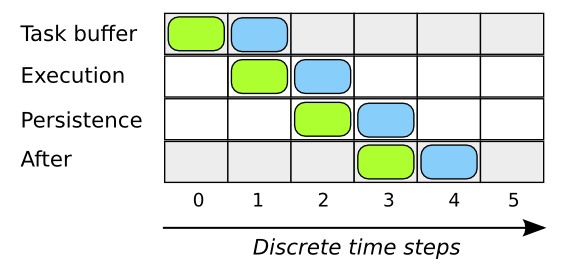
\includegraphics[width=0.5\textwidth]{img/executionPipelineSimple1.png}}\\
\subfloat[Here the persistence step blocks the execution step from fetching in new tasks to execute.]{\label{fig:executionPipelineSimple2}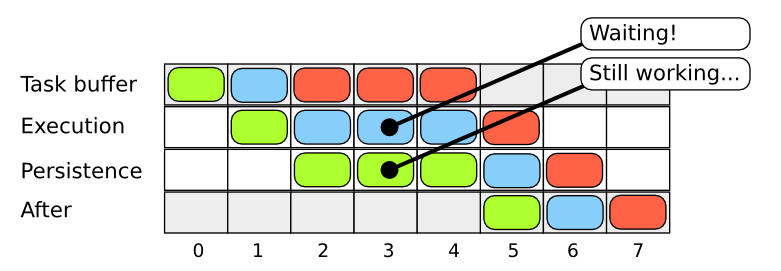
\includegraphics[width=0.7\textwidth]{img/executionPipelineSimple2.png}}
\caption{A simple pipeline helps parallellizing execution and persistance. However, blocking may occur.}
\label{fig:executionPipelineSimple}
\end{figure}In figure \ref{fig:executionPipelineSimple1} a thread starts a transaction,
represented by the green box, at time 0. At time 1, the execution
unit takes the green transaction from the task buffer, and executes
it, while another thread (blue) puts another transaction into the
task buffer. At time 2, the green transaction is handed over to the
persistence unit, while the blue transaction is going into the execution
unit. Now, we can have one thread doing the execution, while another
thread does the persistence. We still return control to the client,
only when the action called by the client has been persisted. Therefore,
the thread issuing the green transaction is blocked, until the green
transaction enters the After slot (only shown for pedagogical reasons).

Each of the two steps in the pipeline are sequentially executed, and
therefore the slowest of them decides the throughput of the complete
pipeline. However, if we add a buffer between the two steps, we can
smooth out the workload of each step, if some transactions are heavier
on the execution and others are heavier on the persistence. The goal
is to keep both the execution and the persistence mechanism as busy
(i.e. non-idling) as possible, with a minimum of waiting. This is
shown on figure~\ref{fig:executionPipelineBetter}. 

\begin{figure}
\centering
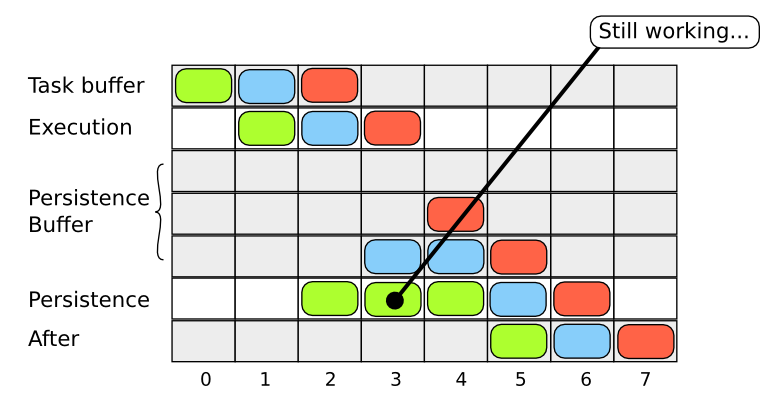
\includegraphics[width=0.7\textwidth]{img/executionPipelineBetter.png}
\caption{By adding a buffer between the execution step, and the persistence step, we can to some extend eliminate blocking of the pipeline.}
\label{fig:executionPipelineBetter}
\end{figure}


\subparagraph{Parallelization of Views}

The second parallelization method takes advantage of the distinction
we have made between the two types of transactions: \emph{actions}
and \emph{views. }Since we know that views can never change the state
of the data model it is safe to parallelize these. It is important
to notice here that even though views have nothing to persist, we
still need to send them through the entire pipeline and not let them
return control to the client thread before they have reached the persistence
step. The reason for this is the \emph{durability} property that we
wish to maintain. We do not want a view to reflect anything in the
data model that has not yet been persisted. If we let the views return
immediately after the execution step, we could get into a situation
where the view reflected the effect of an action that were still in
the persistence buffer, waiting to be persisted. If the persistence
of the action somehow failed, then the view would reflect a non-persisted
state of the data model. Therefore, execution of views is parallelized,
but views must sequentially pass through the persistence unit (which
then does nothing else than marking the view as persisted.)


\subparagraph{The execution algorithm used in the example runtime system}

In EDMA the executor and the persistence module are run in two separate
threads. \emph{Actions} are executed sequentially in the executor
thread while \emph{views }are executed in parallel in their client
threads. The executor has two modes: action-mode and view-mode. When
in action-mode it executes actions in sequence. When in view mode
it lets views execute in their client thread in parallel. When it
switches from view-mode to action-mode, it waits for all current running
views to finish their execution before it starts executing actions.

The pseudo code for the main loop of the executor can be seen in algorithm~\ref{alg:Execution-main-loop}.

\begin{algorithm}[H]
\begin{lstlisting}[tabsize=4]
loop
	t <- get next task from queue
	if(t is an action)
		if(not in action-mode)
			wait for running views to finish
			set mode to action-mode
		executeAction(t)
	else
		set mode to view-mode
		allow t to execute in client thread
\end{lstlisting}


\caption{\label{alg:Execution-main-loop}Execution main loop}
\end{algorithm}


In the current implementation of the executor, a single FIFO queue
is used for both \emph{actions} and \emph{views}. This provides good
fairness, but if \emph{actions} and \emph{views} are highly interleaved,
in the sense that there are no large groups of \emph{views} that are
not interrupted by \emph{actions}, then we do not get much parallelization.
We could instead have two FIFO queues, one for \emph{actions} and
one for \emph{views.} In that way, it would be possible to parallelize
the views in larger chunks. We could then have an algorithm that would
process \emph{views} until the \emph{view} queue is empty and then
switch to process \emph{actions} until the \emph{action} queue is
empty. In order to avoid starvation we could set a maximum number
of transactions to process before looking to the other kind. It is
important to notice here that although this strategy could lead to
a non-chronological execution of transactions, the chronology would
be preserved within each client thread. This is guaranteed, since
whenever a client is executing a transaction, control is never returned
to the client thread before the transaction has been both executed
and persisted.


\paragraph{\label{sub:Persistence}Data Persistence}

In EDMA the current state of the data model is kept in RAM, which
is a volatile storage that is lost in the case of a power failure,
or any other type of system failures. For many applications it is
crucial to store data in a more persistent way so the state of the
data model can be preserved and regenerated even in the case of a
power failure, system reboots an so on. Sometimes it is enough to
store data on a local hard drive, other times applications need a
more secure persistence where data is stored in several different
places.

In EDMA the persistence module is operated on through a simple interface,
making it possible to have different persistence module implementations,
with different strategies for data persistence. Although there is
currently only one implementation, switching between different persistence
strategies can be made into a matter of changing one line of code
for the user. In the following, we describe the strategy that we have
implemented in this project.

Every time an action is executed in EDMA, it generates a sequence
of primitive operations. If the execution fails for some reason, these
operations are rolled back (as described in section \ref{sub:Transactions})
and nothing is sent on to the persistence module. If the action executes
successfully, the sequence of operations that describe all changes
made to the state of the data model instance, is put into an object
called a \emph{persistence unit}. Besides the sequence of operations,
the persistence unit also has two callback functions, one to call
if the data is successfully persisted and another one to call if the
persistence of the data fails for some reason. This persistence unit
is then handed over to the persistence module and whenever the persistence
module has persisted the data or failed in its attempt to do so, it
will call the corresponding callback function on the persistence unit.

This effectively means that every time an action successfully makes
changes to the state of the data model instance, these changes are
persisted as an atomic unit. So when the need for recovery arises,
these changes can be replayed in sequence to re-generate the state.
This also means that a full history of states of the data model is
preserved and could be re-generated if needed.

It is important to note here, that to honor the durability property,
a persistence unit may never be considered successfully persisted
before all preceding persistence units has also been successfully
persisted. Actually \emph{views} also need to pass through the persistence
module as persistence units although they do not have anything to
persist. The reason for this is that the result of a view is not considered
valid or durable before all preceding actions have been successfully
persisted. If the persistence module fails to persist a persistence
unit, then all succeeding persistence units must also be considered
failed, as shown in Figure~\ref{fig:executionPipelineFailing}.

\begin{figure}[h]
	\centering
	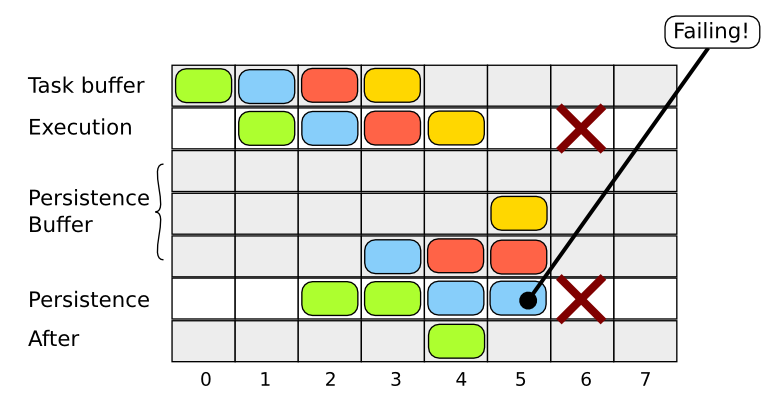
\includegraphics[width=0.7\textwidth]{img/executionPipelineFailing.png}
	\caption{If the persistence module fails, it stops, together with the execution module, and both the task buffer and the persistence buffer is emptied.}
	\label{fig:executionPipelineFailing}
\end{figure}

This may seem like a very bold form of error handling -- shutting
down the whole system, when one thread's transaction fails to be persisted.
However, if the persistence module fails, it means that the disk failed
to write data to the log file, which indicates that there might be
a problem with the disk. Therefore, it wouldn't make sense to continue
writing any subsequent transaction to that file. The failure could
be caused by bad sectors on the disk, which means that it could be
possible to successfully write to a new log file. A clever implementation
of the persistence module (in contrast to our simple proof-of-concept
implementation) could retry writing to the file a number of times,
and upon failure, start writing to a new log file. If that also fails,
writing to another disk could be attempted. Taking it even further,
if writing to any of the disks fails, the system could fall back on
writing to a network socket.

If the system really fails to persist a transaction, EDMA is closed
down, and an administrator will have to manually start the system
again (after running any disk-utility to flag out bad sectors.) Upon
restart, the system reads the whole log file, restoring the data model
to a state identical to the one at the time before the crash.


\subsubsection{SQL Runtime System}

When we planned this thesis, we intended to include a SQL implementation
of the runtime system that would store the data model instances in
a traditional SQL database. 

There are several reasons why this would be a good idea. First, databases
are very mature as a technology, and the database engines are highly
sophisticated and optimized for giving high throughput, serving many
concurrent users, and storing large amounts of data. It would add
some extra work for the user in setting up and connect to a data base,
but this would be rewarded by good scalability in the amount of data
that could be stored. He could always create prototypes with the embedded
java runtime and then switch to the SQL runtime when the need for
storing more data showed up.

However, we chose not to implement an SQL database backed runtime,
because it showed to be more complicated than expected, after we had
invented our value domains system. In an SQL database, there is a
finite set of primitive value domains. In our value domain system,
value domains can be constructed arbitrarily complex, and therefore
there exists an unbounded number of different value domains. This
makes it a non-trivial task to map our entities to SQL tables. It
came to a point where we either had to give up the value domain system
or the SQL implementation due to time constraints.

Given our focus in this project, of investigating the possibilities
of reducing the efforts of coming from a conceptual model to a working
prototype and explore alternative ways of working with data models,
we chose to keep the value domain system and postpone the SQL implementation.


\subsubsection{JDBM3 Runtime System}

The example runtime has the limitation that it can only hold as much
data, as the RAM can contain. Further more, there is a significant
memory footprint in using the example runtime, since all data values
are being wrapped in a number of Java objects, taking up memory (see
the Evaluation section for more details.) For that reason, we have
chosen to exploit the flexibility of the EDMA system, and implemented
the usage of disk-backed sets and maps, using the open source framework
JDBM3. JDBM3 is a key-value store with a number of disk-backed collections,
with the goal of being able to handle billions of items without being
limited by memory. The point of using JDBM3 in EDMA was to have both
large amounts of data, but also to make it possible to perform set
operations on large sets (for results or partial results in actions
and views.)

It turned out that there were some hindrances, making it difficult
to obtain good performance using JDBM3. In order to reach a good performance
level, we need to disable auto-commit in JDBM3. However, having to
manually call commit would require substantial changes in the infrastructure
of the runtime system, therefore complicating the task more than the
benefit added. Further more, it was found that JDBM3 has a bug, preventing
EDMA from using multiple threads access the data store. That said,
since the authors of JDBM3 keep the project alive with frequent updates,
it would be a matter of time before the bug gets fixed.
